    \documentclass[11pt,
        usenames, % allows access to some tikz colors
        dvipsnames % more colors: https://en.wikibooks.org/wiki/LaTeX/Colors
    ]{article}
    \usepackage{
        amsmath,
        amssymb,
        fouriernc, % fourier font w/ new century book
        fancyhdr, % page styling
        lastpage, % footer fanciness
        hyperref, % various links
        setspace, % line spacing
        amsthm, % newtheorem and proof environment
        mathtools, % \Aboxed for boxing inside aligns, among others
        float, % Allow [H] figure env alignment
        enumerate, % Allow custom enumerate numbering
        graphicx, % allow includegraphics with more filetypes
        wasysym, % \smiley!
        upgreek, % \upmu for \mum macro
        listings, % writing TrueType fonts and including code prettily
        tikz, % drawing things
        booktabs, % \bottomrule instead of hline apparently
        xcolor, % colored text
        datetime2
    }
    \usepackage[margin=1in]{geometry} % page geometry
    \usepackage[
        labelfont=bf, % caption names are labeled in bold
        font=scriptsize % smaller font for captions
    ]{caption}
    \usepackage[square, numbers]{natbib}

    \newcommand*{\scinot}[2]{#1\times10^{#2}}
    \newcommand*{\dotp}[2]{\left<#1\,\middle|\,#2\right>}
    \newcommand*{\rd}[2]{\frac{\mathrm{d}#1}{\mathrm{d}#2}}
    \newcommand*{\pd}[2]{\frac{\partial#1}{\partial#2}}
    \newcommand*{\rdil}[2]{\mathrm{d}#1 / \mathrm{d}#2}
    \newcommand*{\pdil}[2]{\partial#1 / \partial#2}
    \newcommand*{\rtd}[2]{\frac{\mathrm{d}^2#1}{\mathrm{d}#2^2}}
    \newcommand*{\ptd}[2]{\frac{\partial^2 #1}{\partial#2^2}}
    \newcommand*{\md}[2]{\frac{\mathrm{D}#1}{\mathrm{D}#2}}
    \newcommand*{\pvec}[1]{\vec{#1}^{\,\prime}}
    \newcommand*{\svec}[1]{\vec{#1}\;\!}
    \newcommand*{\bm}[1]{\boldsymbol{\mathbf{#1}}}
    \newcommand*{\ang}[0]{\;\text{\AA}}
    \newcommand*{\mum}[0]{\;\upmu \mathrm{m}}
    \newcommand*{\at}[1]{\left.#1\right|}
    \newcommand*{\bra}[1]{\left<#1\right|}
    \newcommand*{\ket}[1]{\left|#1\right>}
    \newcommand*{\abs}[1]{\left|#1\right|}
    \newcommand*{\ev}[1]{\left\langle#1\right\rangle}
    \newcommand*{\p}[1]{\left(#1\right)}
    \newcommand*{\s}[1]{\left[#1\right]}
    \newcommand*{\z}[1]{\left\{#1\right\}}

    \newtheorem{theorem}{Theorem}[section]

    \let\Re\undefined
    \let\Im\undefined
    \DeclareMathOperator{\Res}{Res}
    \DeclareMathOperator{\Re}{Re}
    \DeclareMathOperator{\Im}{Im}
    \DeclareMathOperator{\Log}{Log}
    \DeclareMathOperator{\Arg}{Arg}
    \DeclareMathOperator{\Tr}{Tr}
    \DeclareMathOperator{\E}{E}
    \DeclareMathOperator{\Var}{Var}
    \DeclareMathOperator*{\argmin}{argmin}
    \DeclareMathOperator*{\argmax}{argmax}
    \DeclareMathOperator{\sgn}{sgn}
    \DeclareMathOperator{\diag}{diag\;}

    \colorlet{Corr}{red}

    % \everymath{\displaystyle} % biggify limits of inline sums and integrals
    \tikzstyle{circ} % usage: \node[circ, placement] (label) {text};
        = [draw, circle, fill=white, node distance=3cm, minimum height=2em]
    \definecolor{commentgreen}{rgb}{0,0.6,0}
    \lstset{
        basicstyle=\ttfamily\footnotesize,
        frame=single,
        numbers=left,
        showstringspaces=false,
        keywordstyle=\color{blue},
        stringstyle=\color{purple},
        commentstyle=\color{commentgreen},
        morecomment=[l][\color{magenta}]{\#}
    }

\begin{document}

\pagestyle{fancy}
\lhead{Compiled at: \DTMnow}
\rfoot{Yubo Su}
\rhead{}
\cfoot{\thepage/\pageref{LastPage}}

\title{Guest Lecture: Spin-Orbit Resonance and Resonance Capture}
\author{Yubo Su}
\date{Apr 11, 2024}

\maketitle

\textbf{Note from the author:} Hey guys, just wanted to provide a set of
reference notes for y'all, since the lecture could have been significantly
clearer, and some of these concepts are simple enough that they're worth
remembering. I've structured the notes with a general overview section (I swear
it's shorter than it looks) with just a few bullet-pointed ideas, and then
leave the algebra for the later sections. I hope this helps recapitulate
everything we talked about a bit, and I'm sorry for the delay!

\section{Overview}

In this lecture, we covered three concepts from planetary dynamics: (i)
spin-orbit resonance [non-secular], (ii) ``secular spin-orbit resonance'', and
(iii) dissipative resonance capture. A few key ideas to contextualize and
summarize our discussion:
\begin{itemize}
    \item (Non-secular) Spin-Orbit Resonance
        \begin{itemize}
            \item Key idea: ``When the planet is slightly aspherical and
                elongated, its long axis wants to point towards the host star.''

            \item Developed mathematically, this long axis oscillates much like
                a pendulum, with the lowest energy state being permanent
                alignment along the star-planet axis (pendulum pointing down).
                This is the 1:1 spin-orbit resonance, where the spin frequency
                $\Omega_{\rm s}$ of the planet equals its mean motion $n$
                (orbital frequency).

            \item This can be generalized to eccentric orbits, and pendulum-like
                equilibria/resonances occur when $\Omega_{\rm s} / n = k/2$, for
                integer $k$.

                This is the cause of Mercury's famous 3:2 spin
                orbit resonance, where it rotates three times for every two
                orbits around the Sun: Mercury is eccentric and has a long axis
                (in the equatorial plane) that tries to point towards the host
                star.
        \end{itemize}

    \item Secular Spin-Orbit Resonance
        \begin{itemize}
            \item Key idea: ``When a planet has an equatorial bulge and also has
                a misaligned companion planet, its spin axis wants to remain in
                the plane of the two planets' orbit normals.''

            \item Recall that, in the \emph{secular approximation}, we aim to
                study long-term behavior of planetary dynamics by averaging over
                the spin and orbital phases of the planet.

            \item In this approximation, a rotating planet (which will exhibit
                an equatorial bulge) orbiting its host star will experience
                \emph{spin precession}.

                Because the star gravitationally tugs on the equatorial bulge,
                this results in a torque that causes the spin vector to
                ``precess'' about the planet's orbit normal.

            \item At the same time, if the planet has a distant, massive
                companion planet with a misaligned orbit (the orbits are not
                coplanar), then the planet will undergo \emph{orbital
                precession}.

                This is because the ``ring of mass'' (orbit averaged) of the
                outer companion tugs on the ``ring of mass'' of the inner
                planet, causing the orbit normal of the inner planet to precess
                about that of the outer planet (to be precise, they precess
                about the axis of their combined angular momentum).

            \item If the system configuration is such that these two precession
                frequencies match, then the planet's spin, planet's orbit, and
                companion's orbit will precess such that they remain in the same
                plane (alternatively, the planet's spin is fixed in the frame
                co-precessing with the orbit precession).

                Such configurations are called \emph{Cassini States}.

            \item For certain ratios of precession frequencies, one of the
                Cassini States is surrounded by a pendulum-like region of phase
                space, hence ``secular spin-orbit resonance.''
        \end{itemize}

    \item Resonance Capture
        \begin{itemize}
            \item Resonance capture refers to the process by which a system
                transitions from circulation (a pendulum swinging
                [counter]clockwise) to libration within a resonance (a pendulum
                oscillating about a downwards orientation).

            \item The old theory (an earlier lecture in the class) suggests that
                resonance capture is a process that can be understood for
                Hamiltonian systems that are varied adiabatically (e.g.\ a
                pendulum whose length is slowly changed).

            \item Through a careful analysis of critical orbits, we show that
                resonance capture can also be understood for near-Hamiltonian
                systems that are Hamiltonian except for a small perturbation
                (e.g.\ a pendulum with air resistance; spin-orbit resonance with
                tidal obliquity damping).
        \end{itemize}
\end{itemize}

\section{The Story}

No, this is not ``the story'' that I told in class, which I remain grateful for
everybody's laughter.

Consider a planet with mass $M \gtrsim$ that of the Earth and radius $R$ in
orbit around a star with $M_\star = M_\odot$ on a circular orbit with semimajor
axis $a \lesssim 1\;\mathrm{AU}$. At such separations, the planet will evolve
towards a tidally locked state (spin frequency = orbital frequency, spin axis
aligned with orbit normal) on timescales $\lesssim \;\mathrm{Gyr}$, less than
the age of most observed planetary systems.

Suppose that exterior to this planet, a Jupiter-like planet ($M_{\rm p} \sim
M_{\rm Jup}$ at $a_{\rm p} \sim 5\;\mathrm{AU}$) is on an orbit inclined to the
inner planet's orbit by the mutual inclination $I$.

We expect that planets may form with large ``obliquities'', the angle between
the planet's spin and orbital axes. As tides act to damp the large primordial
obliquity of the inner planet, its obliquity sometimes is trapped at $\sim
90^\circ$. In this lecture, we will explore this process a bit.

The first section, on non-secular spin-orbit resonances, is not relevant for
this story, but is included for historical completeness, since it is important
in the solar system and is a little more intuitive.

\section{Non-Secular Spin-Orbit Resonances}

\textbf{The physical idea here is clear}: an elongated planet wants to point its long
axis towards its host star (see left hand side of Fig.~\ref{fig:res}).
Conceivably, this is similar to a pendulum, which wants to point downwards. How
can we show this mathematically?
\begin{figure}
    \centering
    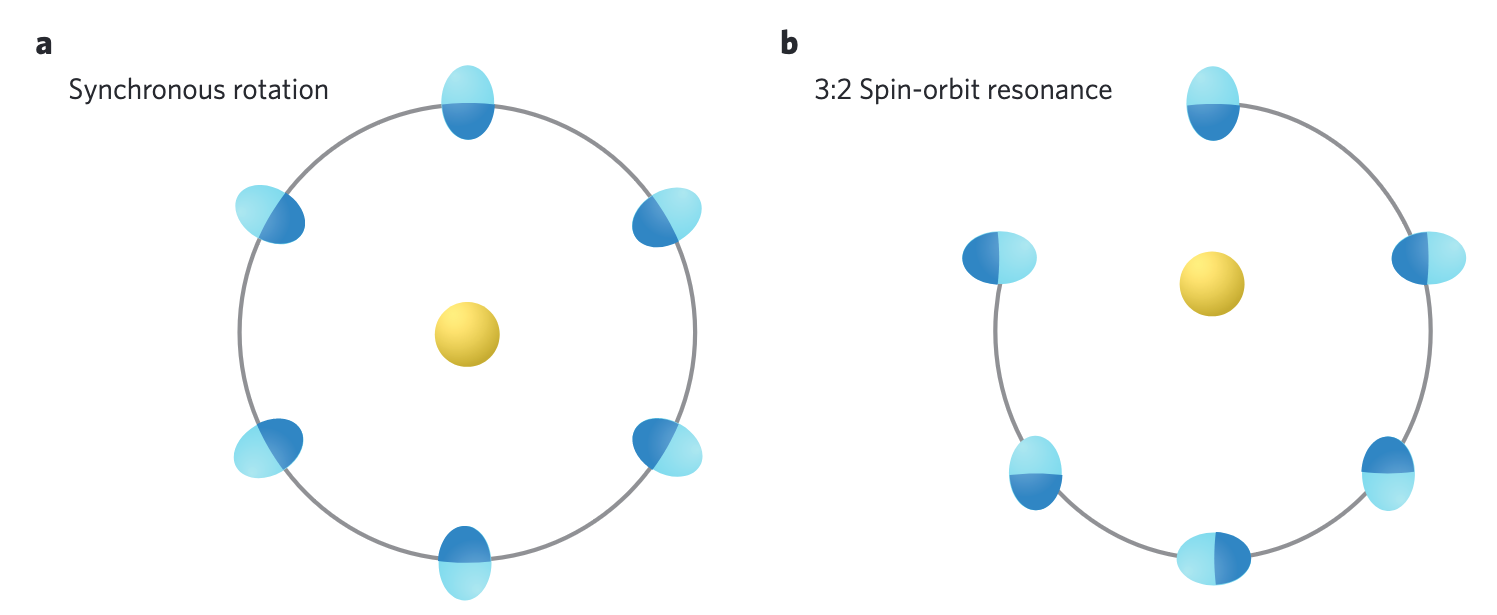
\includegraphics[width=0.5\columnwidth]{res.png}
    \caption{(left) 1:1 spin orbit resonance. (right) Mercury's spin-orbit
    resonant state \citep{cuk2012kick}.}\label{fig:res}
\end{figure}

Before we start, note that this is traditionally what people mean when they talk
about spin-orbit resonance, since it's literally a commensurability of the spin
and orbital frequencies. In exoplanetary dynamics, we've only recently started
being able to put direct observational constraints on planetary spin phase, so
we typically study secular spin-orbit resonances, described in the next section,
and will involve a commensurability of the spin and orbital secular
\emph{precession} frequencies instead.

We start by writing down the Hamiltonian governing the spin evolution of the
planet. This consists of its rotational kinetic energy as well as the
gravitational potential energy of the body, which is the quadrupolar tidal
potential to leading order. The potential energy is given by \emph{MacCullagh's
Formula} (Tremaine Eq.~1.129 \& 7.25), and we arrive at:
\begin{equation}
    H_{\rm spin} = \frac{1}{2}\p{
        \vec{\Omega}_{\rm s} \cdot \bm{I} \cdot \vec{\Omega}_{\rm s}
        + 3\frac{GM_\star}{r^3}\hat{r} \cdot \bm{I} \cdot \hat{r}
        - \frac{GM_\star}{r^3}\Tr\p{\bm{I}}}.\label{eq:Hspin}
\end{equation}
Here, $\vec{\Omega}_{\rm s}$ is the spin vector of the planet, $M_\star$ is the mass of
the host star, $r$ is the distance from the planet to the host star, $\hat{r}$
is the separation direction from the host star, and
\begin{equation}
    \bm{I}
        = \int \vec{R}\vec{R}\;\mathrm{d}m
        = \begin{pmatrix}
            A&0&0\\
            0&B&0\\
            0&0&C
        \end{pmatrix}_{\hat{\imath}\hat{\jmath}\hat{k}},
\end{equation}
is the planet's moment of inertia matrix ($\vec{R}$ labels position inside the
planet), and we've written its components in its principal axis basis. Here, $A
\leq B \leq C$, and $C$ is the moment of inertia about $\hat{k}$, the shortest
principal axis and the one with the largest moment of inertia.

Note that the last term of Eq.~\eqref{eq:Hspin} does not affect the spin
dynamics, as it is spherically symmetric, and only modifies the radial motion of
the planet; thus we can ignore it going forward.

\subsection{Circular}

For simplicity, let's assume the planet's orbit is circular and its spin is
along $\hat{k}$ and is aligned with the orbit normal (zero ``obliquity'', so
$\hat{r} \cdot \hat{k} = 0$), i.e.\ the planet's equator lies in its orbital
plane. Then Eq.~\eqref{eq:Hspin} simplifies to
\begin{equation}
    H_{\rm spin} =
        \frac{C\Omega_{\rm s}^2}{2} + \frac{3n^2}{2}
            \s{A\p{\hat{r} \cdot \hat{\imath}}^2 + B\p{\hat{r} \cdot
            \hat{\imath}}^2},
            \label{eq:Hspin_coplanar}
\end{equation}
where $n^2 = GM_\star/a^3$ is the mean motion / orbital angular frequency. But
of course, $\p{\hat{r} \cdot \hat{\imath}}^2 = 1 - \p{\hat{r} \cdot
\hat{\imath}}^2$, so we can rewrite, dropping another overall constant
\begin{equation}
    H_{\rm spin}
        = \frac{C\Omega_{\rm s}^2}{2} + \frac{3n^2(B - A)}{2}
            \p{\hat{r} \cdot \hat{\imath}}^2.
\end{equation}
Now, if $f = nt$ is the planet's true anomaly (uniformly advances at rate $n$),
and $\phi$ is the spin phase of the planet ($\dot{\phi} = \Omega_{\rm s}$), then
(again, subtracting out a constant)
\begin{equation}
    H_{\rm spin}
        = \frac{C\Omega_{\rm s}^2}{2} - \frac{3n^2(B - A)}{4}\cos2\p{\phi - nt}.
\end{equation}
It is quite clear that $H\p{\Omega_{\rm s}, \phi - nt}$ looks almost like a pendulum ($H
\sim \dot{\theta}^2/2 - \cos\theta$) except that there are two stable
equilibria, $\phi = nt$ and $\phi = nt + \pi$. This has a simple interpretation:
a planet doesn't care whether its $\hat{\imath}$ axis is aligned or antialigned
with $\hat{r}$, the potential will be the same.

\subsection{Eccentric}

See Murray \& Dermott \S5.4 or Tremaine \S7.2 for a more careful derivation; we
will just try to identify the key intuition behind the claim ``spin-orbit
resonances exist at half-integer ratios of $\Omega_{\rm s} / n$.''

The above procedure can be easily generalized to handle an eccentric planet,
though we will focus on the zero-obliquity case again for now. We return to
Eq.~\eqref{eq:Hspin} and obtain instead a slightly modified version of
Eq.~\eqref{eq:Hspin_coplanar}:
\begin{equation}
    H_{\rm spin}
        = \frac{C\Omega_{\rm s}^2}{2} + \frac{3GM_\star(B - A)}{2r^3}
            \p{\hat{r} \cdot \hat{\imath}}^2.
\end{equation}
In an eccentric orbit, $\hat{r}$ no longer advances uniformly with time.
Instead, the components in the inertial frame $\hat{r}_x = \cos f$ and
$\hat{r}_y = \sin f$ can be expressed as a Fourier series in the
\emph{mean anomaly} $\mathcal{M} = nt$, which does advance uniformly (e.g.\ Murray \&
Dermott Eqs.~2.84--2.85). This result is quite messy, but broadly speaking:
\begin{align}
    \hat{r} &= \s{\sum\limits_{p=0}^\infty P_p \cos k\mathcal{M}} \hat{x}
        + \s{\sum\limits_{q=1}^\infty Q_q \sin q\mathcal{M}} \hat{y},\\
    \hat{\imath} &= \cos \phi \hat{x} + \sin \phi \hat{y},\\
    H_{\rm spin}
        &= \frac{C\Omega_{\rm s}^2}{2} + \frac{3GM_\star(B - A)}{2r^3}
            \p{\hat{r} \cdot \hat{\imath}}^2\nonumber\\
        &= \frac{C\Omega_{\rm s}^2}{2} + \frac{3GM_\star(B - A)}{2r^3}
            \times \s{(\dots) - \sum\limits_{p=0}^\infty
            \sum\limits_{q=1}^\infty
                F_{pq} \cos\p{(p + q)\mathcal{M} - 2\phi}
                + G_{pq} \cos\p{(p + q)\mathcal{M} + 2\phi}}
                .\label{eq:H_spin_ecc}
\end{align}
The terms are a bit laborious to evaluate out by hand, but the principle of it
is clear: we dot the $x, y$ components of $\hat{r}$ and $\hat{\imath}$, then
product-to-sum identities give us some coefficient $F_{pq}$ (which depends on
the Fourier coefficients $P_p$ and $Q_q$) multiplied by cosines with the correct
arguments, plus a bunch of extra terms (denoted with the ``\dots'') that do not
have the correct trig argument.

\textbf{This may look complicated, but the upshot is this}: the potential energy
term in $H_{\rm spin}$ has a bunch of pendulum-like terms. Each of these angles
can ``librate'' (like pendulum pointing down, where its phase will oscillate
about the downward-pointing value), and if so, the system is trapped in this
resonance. The set of possible resonant angles is $(p+q)\mathcal{M} \pm 2\phi$
(this angle is called $2\gamma$ in Murray \& Dermott) for $p \geq 0$ and $q \geq
1$, so librating resonant angles can appear when
\begin{equation}
    kn = 2\Omega_{\rm s},
\end{equation}
for integer $k$. This is as expected. \textbf{In these resonances, the planet's
long axis should point at the host star at pericenter}, also as expected. For $k
= 3$, this yields the essence of Mercury's 3:2 spin-orbit resonance (see
Fig.~\ref{fig:res}).

NB\@: The standard formulation just directly presents the coefficients for
different values of $k$ above, e.g.\ see Murray \& Dermott (5.73--5.82) or
Tremaine (7.32). For practical use, that is much more direct and suffices, but
it's useful to convince ourselves where the coefficients come from.

\section{Secular Spin-Orbit Resonance}

\textbf{The physical idea here is a little less obvious, but can be concisely
stated:} In a 2-planet system where the planetary orbits are not coplanar, and
if a planet's obliquity (denoted $\theta \equiv \arccos \hat{\Omega}_{\rm s}
\cdot \hat{l}$) is at the right value, then the planet's spin will tend to want
to align with the plane containing the two planets' orbit normals. This effect
happens due to \emph{secular} precession frequencies, dynamics arising after
averaging over the spin and orbits of the planets.

Note that most of this disussion follows \citet{su2022dynamics}, which is a very
physically motivated discussion of ``Colombo's Top'', the simplest model for
secular spin-orbit resonance. This is an old system though, dating back to
\citet{colombo1966cassini, henrard1987colombo} as some classic references that
approach this from a very celestial-mechanics point of view. Scott Tremaine's
textbook also covers this in Chapter 7.

For simplicity, we will assume that all orbits are circular, though the
derivations are not too significantly altered if the orbits are eccentric.

\subsection{Precession Equations}

First, we need to briefly discuss our planetary model. Most commonly, a planet
is modeled as a self-gravitating, rotating fluid. Thus, the fluid satisfies
hydrostatic equilibrium, including the centrifugal potential, and will bulge
slightly at the equator. This has two ramifications for spin dynamics: (i) $A =
B < C$, where $A=B$ because the planet is axially symmetric about its short
polar axis $\hat{k}$ (we call this ``oblate''); and (ii) $\hat{\Omega}_{\rm s} =
\hat{k}$, i.e.\ the planet spins about its polar axis\footnote{Fun dynamics
occur when considering the spin evolution of satellites or rocky planets, see
\citet{gladman1996synchronous} or a submitted paper by Yuan, Su, \& Goodman
2024.}. In particular, because the centrifugal potential $\propto \Omega_{\rm
s}^2$, it is a textbook exercise to show that
\begin{equation}
    \frac{C - A}{MR^2} \propto \Omega_{\rm s}^2.
\end{equation}
To be more precise, the often used relationship is
\begin{equation}
    J_2 \equiv \frac{C - A}{MR^2} = \frac{k_2}{3}\frac{\Omega_{\rm
    s}^2}{GM/R^3},
\end{equation}
where $k_2$ is the ``second Love number'' (an order-unity number quantifying how
centrally concentrated a body's mass is---for a body of uniform density, $k_2 =
1.5$, while for planets it is typically $\sim 0.5$--$1$) and $M$ and $R$ are the
planet's mass and radius. This scaling makes sense: if the rotation rate is of
order the dynamical infall rate $\sqrt{GM/R^3}$, then the planet's rotational
flattening is of order unity.

How does this lead to spin precession? Well, the gravitational potential
component of the spin Hamiltonian for an oblate planet (no longer assuming zero
obliquity) reads:
\begin{align}
    V_{\rm spin} &= \frac{3n^2}{2}\hat{r} \cdot \bm{I} \cdot \hat{r}\nonumber\\
        &= \frac{3n^2}{2}\s{r_i^2A + r_j^2B + r_k^2C},
\end{align}
where $r_i \equiv \hat{r} \cdot \hat{\imath}$ etc.\ (I'll try to refrain from
using this shorthand for the most part). Then, since $B = A$, and $r_i^2 + r_j^2
+ r_k^2 = 1$, we can subtract out a constant to obtain
\begin{equation}
    V_{\rm spin} = \frac{3n^2(C - A)}{2}\p{\hat{r} \cdot \hat{k}}^2.
\end{equation}

Next, we want to get from this potential to spin precession, for which there are
multiple methods, see Tremaine \S7.1 for an alternative option. Here's a coarse
idea. Now, if the planet has zero obliquity, then $\hat{r}$ (in the orbital
plane) also lies along the equator of the planet, and $\hat{r} \cdot \hat{k} =
0$, while if the planet's obliquity is exactly $90^\circ$, then $\hat{r} \cdot
\hat{k}$ varies sinusoidally between $[-1, 1]$, and its square time-averages to
$1/2$. Thus, it's an easy guess (and can be verified; Tremaine Eq.~7.3) that
\begin{equation}
    \ev{V_{\rm spin}}
        = \frac{3n^2(C - A)}{4}\p{\hat{l} \cdot \hat{k}}^2
        = \frac{3n^2(C - A)}{4}\p{\hat{l} \cdot \hat{\Omega}_{\rm s}}^2,
\end{equation}
where I've replaced $\hat{k} = \hat{\Omega}_{\rm s}$. I'll drop the angle
brackets, which denote secular averaging, going forwards.

To understand the evolution of the spin axis, we apply the following:
\begin{equation}
    \rd{\hat{\Omega}_{\rm s}}{t}
        = -\frac{1}{S}\nabla_{\hat{\Omega}_{\rm s}}V_{\rm
        spin},\label{eq:nablaS}
\end{equation}
where $S \equiv C\Omega_{\rm s}$ is the magnitude of the spin angular momentum.
This has many interpretations, all of which analyze the torque the point-mass
host star experiences, two of which are: it's a torque on the host star
(Tremaine 7.2), or it's an application of the Milankovich Equations (but for a
circular orbit).

\textbf{Somewhat laboriously, we've arrived at one of the results from
\citet{su2022dynamics}}, Eq.~(1):
\begin{align}
    \rd{\hat{\Omega}_{\rm s}}{t}
        &= \omega_{\rm sl}\p{\hat{\Omega}_{\rm s} \cdot
        \hat{l}}\p{\hat{\Omega}_{\rm s} \times \hat{l}},\label{eq:dsdt1}\\
    \omega_{\rm sl} &\equiv \alpha =
        \frac{3n^2(C - A)}{2C\Omega_{\rm s}}
            \label{eq:wsl}.
\end{align}
This spin precession frequency is commonly denoted $\alpha$ in the literature.

I'll not belabor the orbital precession: two mutually inclined planets will
experience orbital precession about their combined angular momentum axis
(secular Laplace-Lagrange theory, which was covered earlier in the course;
Tremaine S5.2). If the outer planet has much more angular momentum than the
inner planet (as in our canonical story), then the dynamics can be approximated
as precession of the inner planet $\hat{l}$ about the perturbing outer planet
$\hat{l}_{\rm p}$:
\begin{align}
    \rd{\hat{l}}{t} &= \omega_{\rm lp}\p{\hat{l} \cdot \hat{l}_{\rm p}}\p{\hat{l}
        \times \hat{l}_{\rm p}} \equiv -g\p{\hat{l} \times \hat{l}_{\rm p}},
        \label{eq:dldt1}\\
    \omega_{\rm lp} &\equiv -\frac{g}{\cos I}
        = \frac{3M_{\rm p}}{4M_\star}\p{\frac{a}{a_{\rm p}}}^3 n.\label{eq:wlp}
\end{align}
The precession frequency $g < 0$ is often defined for reasons unclear to me.

Eqs.~(\ref{eq:dsdt1}--\ref{eq:dldt1}) describe the mutual motion of the two
vectors $\hat{\Omega}_{\rm s}$ and $\hat{l}$ with reference to the fixed vector
$\hat{l}_{\rm p}$.

\subsection{Secular Spin-Orbit Resonance: Cassini States}

One nice insight is that, since $\hat{l}$ precesses uniformly about
$\hat{l}_{\rm p}$, we can perform a change of reference frame to co-precess with
$\hat{l}$ about $\hat{l}_{\rm p}$:
\begin{align}
    \p{\rd{\hat{l}}{t}}_{\rm rot} &= 0,\\
    \p{\rd{\hat{\Omega}_{\rm s}}{t}}_{\rm rot}
        &= \alpha\p{\hat{\Omega}_{\rm s} \cdot \hat{l}}
            \p{\hat{\Omega}_{\rm s} \times \hat{l}}
            + g\p{\hat{\Omega}_{\rm s} \times \hat{l}_{\rm
            p}}.\label{eq:dsdt_rot}
\end{align}
In talks, I like to call this trick ``I'm a lazy dynamicist, and two moving
vectors is one too many.''

\textbf{Cassini States:} next, we identify the equilibria of
Eq.~\eqref{eq:dsdt_rot}. These spin states are where $\hat{\Omega}_{\rm s}$ is
fixed in the co-precessing frame. In the inertial frame, $\hat{\Omega}_{\rm s}$
remains in a fixed orientation with $\hat{l}$ and $\hat{l}_{\rm p}$; as we shall
soon see, Cassini States (CSs) for $\hat{\Omega}_{\rm s}$ are actually coplanaar with
the $\hat{l}$--$\hat{l}_{\rm p}$ plane.

We begin with a simple qualitative analysis, in the two limiting cases where $g
\ll \alpha$ and where $g \gg \alpha$, as illustrated in Fig.~\ref{fig:cs_limits}:
\begin{itemize}
    \item In the former case, spin equilibria occur
          whenever $\p{\hat{\Omega}_{\rm s} \cdot \hat{l}} = 0$ or when
          $\p{\hat{\Omega}_{\rm s} \times \hat{l}} = 0$; this implies two CSs
          with $\hat{\Omega}_{\rm s} \parallel \hat{l}$ and two with
          $\hat{\Omega}_{\rm s} \perp \hat{l}$.

    \item In the latter case, spin equiibria only occur when $\hat{\Omega}_{\rm
        s} \parallel \hat{l}_{\rm p}$. Thus, there are only two CSs in this
        limit.
\end{itemize}
\begin{figure}
    \centering
    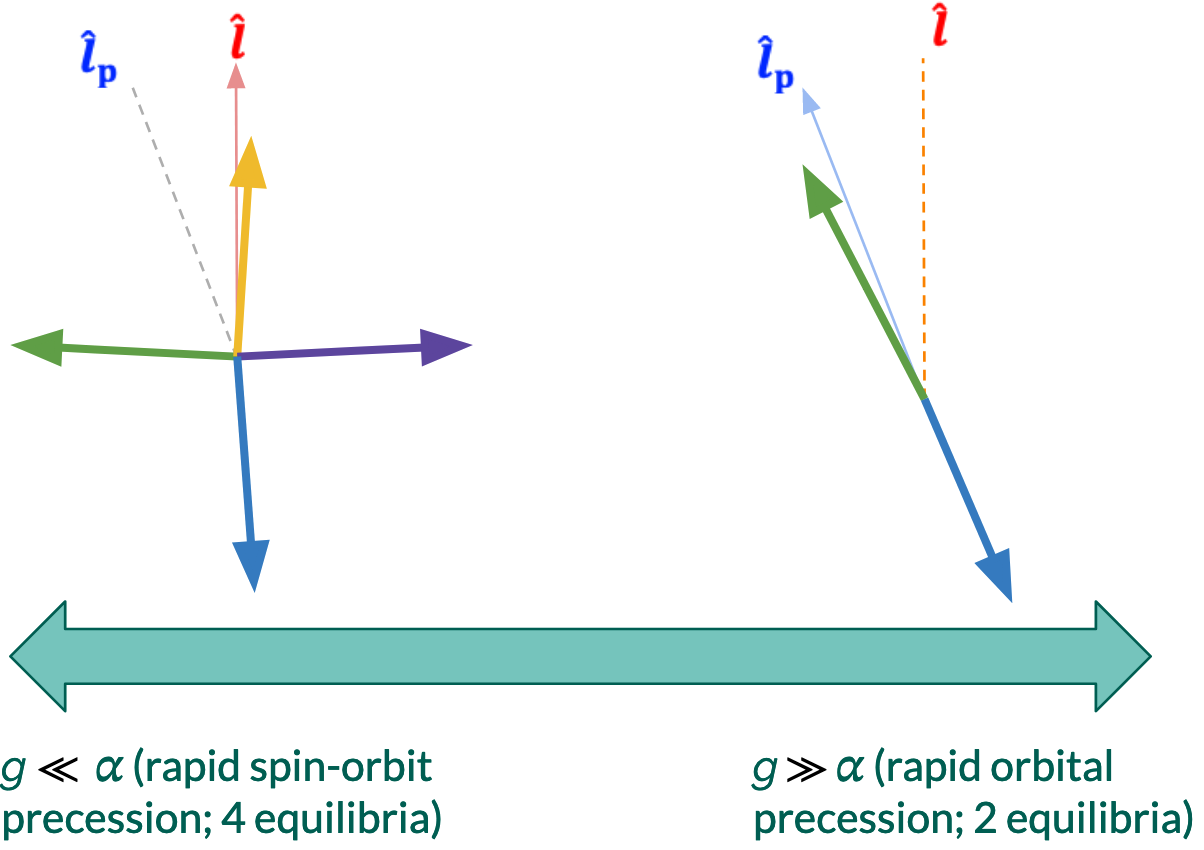
\includegraphics[width=0.5\columnwidth]{cs_limits.png}
    \caption{Locations of the Cassini States (spin equilibria) in the two limits
    $g \ll \alpha$ and $g \gg \alpha$. Note that CS1 and CS2 are stable
    (``centers'' in the dynamical systems language) as long
    as the tidal dissipation is sufficiently small, but CS3 is only stable if
    tidal dissipation is exactly zero. CS4 is a saddle
    point.}\label{fig:cs_limits}
\end{figure}

To do this more quantitatively, we adopt a spherical coordinate system in the
co-precessing frame such that $\hat{z} = \hat{l}$, $\hat{l}_{\rm p} \times
\hat{l} \propto \hat{y}$, and the spherical coordinates are the polar angle
$\theta$ and the azimuthal angle $\phi$. For convenience going forward,
we rescale time such that $\tau = \alpha t$ and
\begin{equation}
    \eta \equiv -\frac{g}{\alpha}.\label{eq:etadef}
\end{equation}
Then the equations of motion are
\begin{align}
    \rd{\theta}{\tau} &= \eta\sin I \sin \phi \label{eq:dqdt_toy}\\
    \rd{\phi}{\tau} &= - \cos\theta
        + \eta\p{\cos I + \sin I \cot \theta \cos \phi},\label{eq:dfdt_toy}
\end{align}
where $I = \arccos\p{\hat{l} \cdot \hat{l}_{\rm p}}$ is the mutual inclination.
The solutions to this system are shown in Fig.~\ref{fig:cs_locs}. It can be
shown that the number of CSs changes from $2$ to $4$ when $\eta$ crosses the
critical value
\begin{equation}
    \eta_{\rm c} \equiv \p{\sin^{2/3}\!I + \cos^{2/3}\!I}^{-3/2}.
        \label{eq:def_etac}
\end{equation}
\begin{figure}
    \centering
    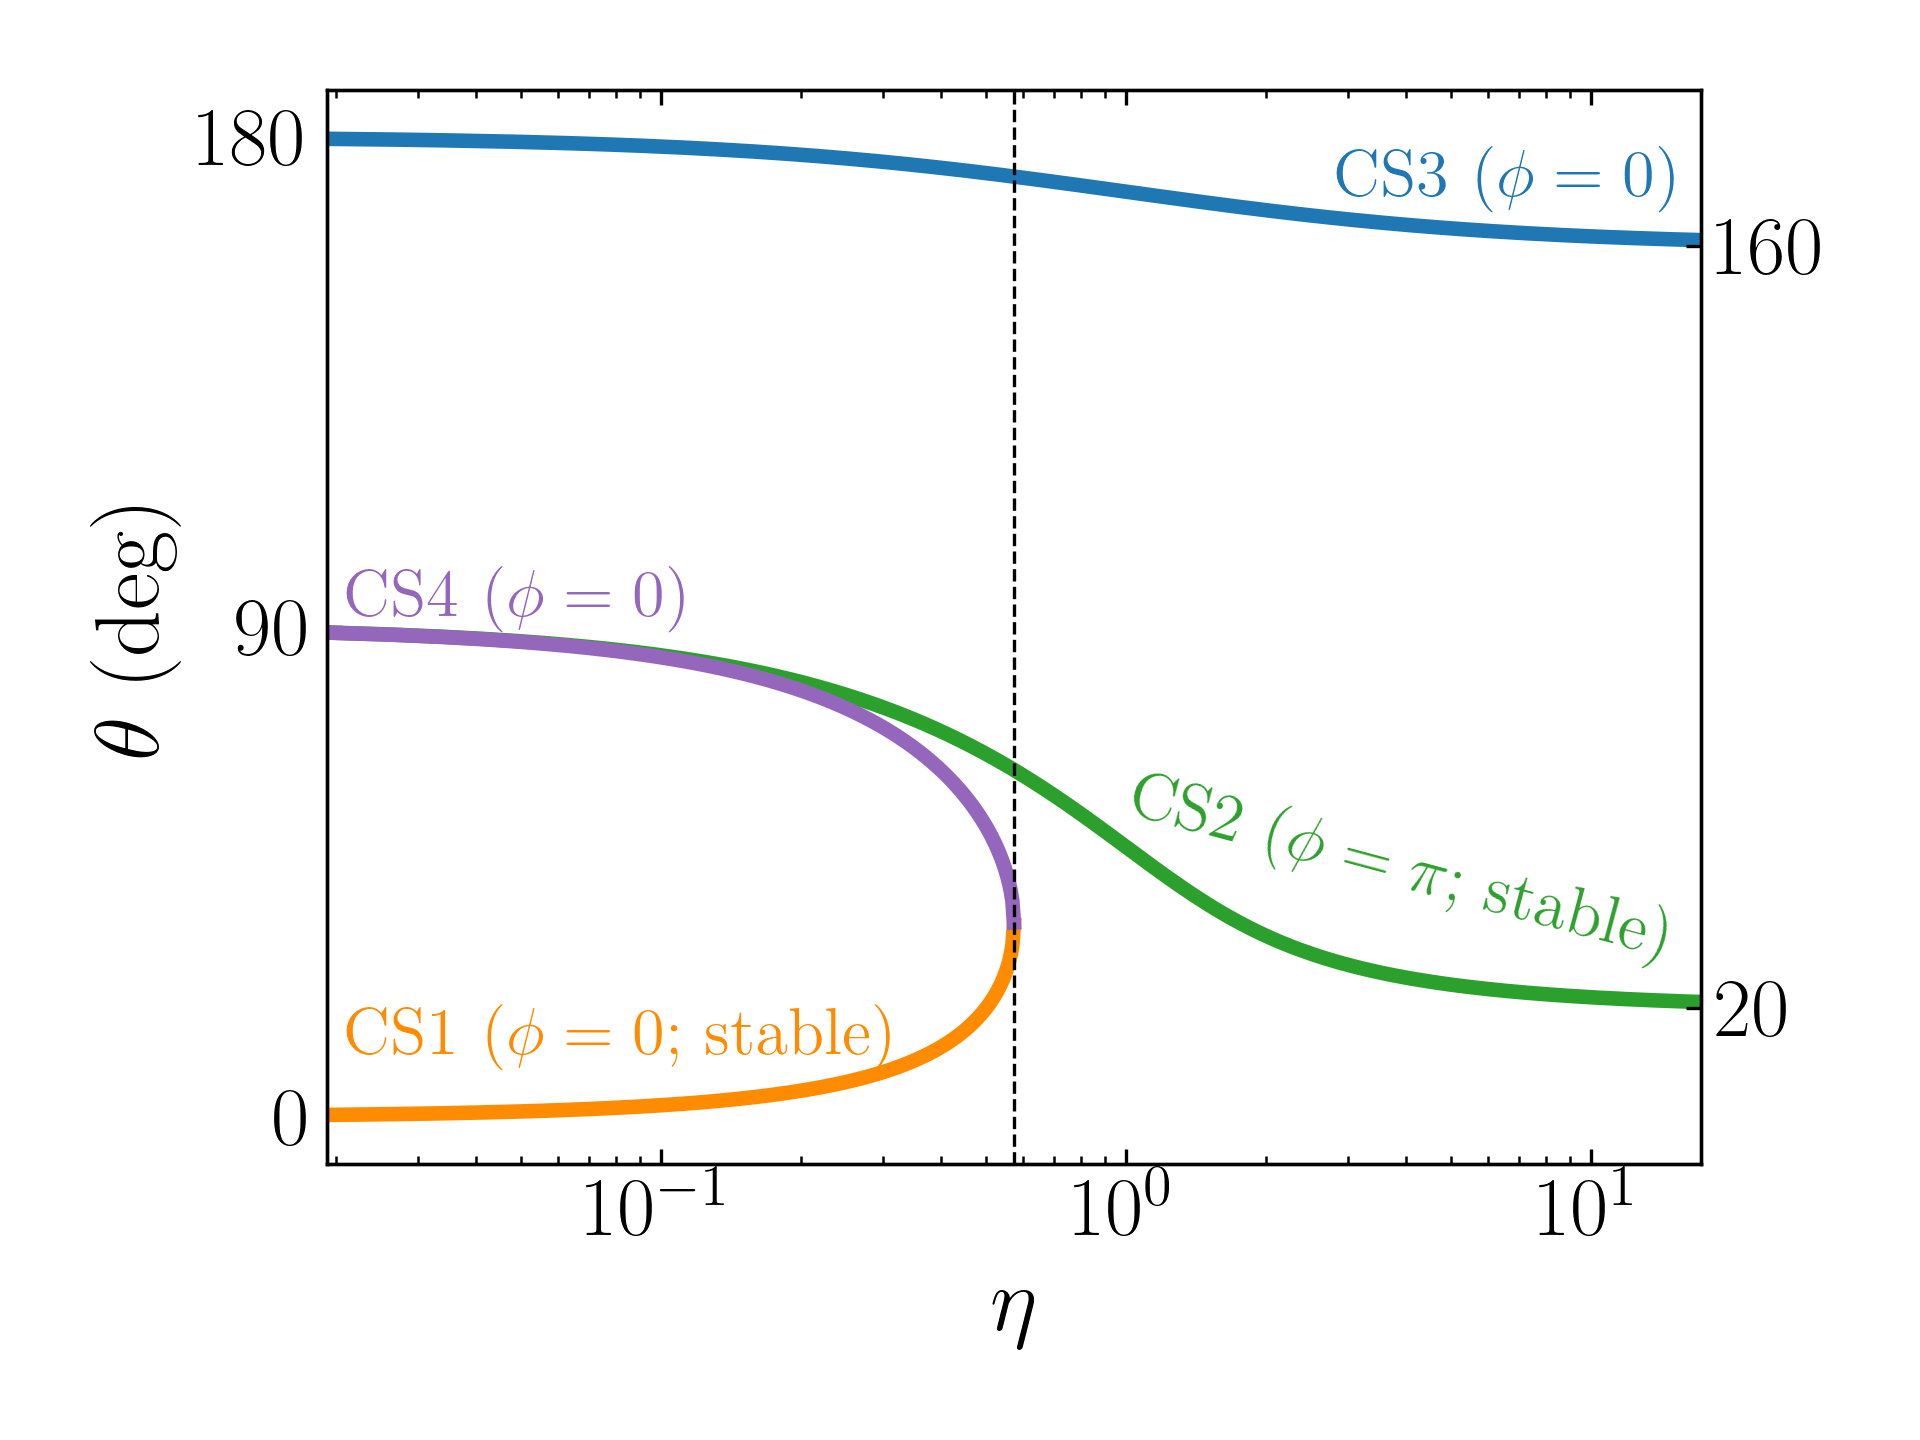
\includegraphics[width=0.5\columnwidth]{2_cs_locs_phi.png}
    \caption{Locations of the Cassini States for $I = 20^\circ$, the equilibria
    to Eqs.~(\ref{eq:dqdt_toy}--\ref{eq:dfdt_toy}), where $\eta = -g/\alpha$
    (Eq.~\ref{eq:etadef}). Note the agreement, in terms of the number of CSs,
    with Fig.~\ref{fig:cs_limits}. The vertical line is $\eta_{\rm c}$ given by
    Eq.~\eqref{eq:def_etac}.}\label{fig:cs_locs}
\end{figure}

Finally, to see the resonant structure of the CS equilibria, it is easiest to
directly plot the level curves of the Hamiltonian. In terms of the rescaled
coordinates,
\begin{align}
    H &= -\frac{1}{2}\p{\hat{\Omega}_{\rm s} \cdot \hat{l}}^2
            + \eta\p{\hat{\Omega}_{\rm s} \cdot \hat{l}_{\rm p}}\nonumber\\
    H(\cos\theta, \phi) &= -\frac{1}{2} \cos^2\theta
            + \eta\p{\cos\theta \cos I - \sin I \sin\theta \cos \phi},\label{eq:H}
\end{align}
where we've expressed $H$ in terms of the canonically conjugate coordinates
$(\cos\theta, \phi)$\footnote{That these two are canonically conjugate is not
immediately obvious, but when considering the orbit of the Sun in the spin-frame
of the planet, the Delaunay variables $G\cos i, \Omega$ are conjugate, which
translates to $\cos\theta, \phi$ in the inertial frame when $G$ is constant.
Alternatively, this is the condition necessary for Eq.~\eqref{eq:nablaS} to
work.}
The level curves for this, in terms of $\eta$, are shown in
Fig.~\ref{fig:contours}. \textbf{Note that when $\eta < \eta_{\rm c}$, and there
are four CSs, that the green point (``Cassini State 2'') is surrounded by a
separatrix, and is reminiscent of a pendulum's phase space.}
\begin{figure}
    \centering
    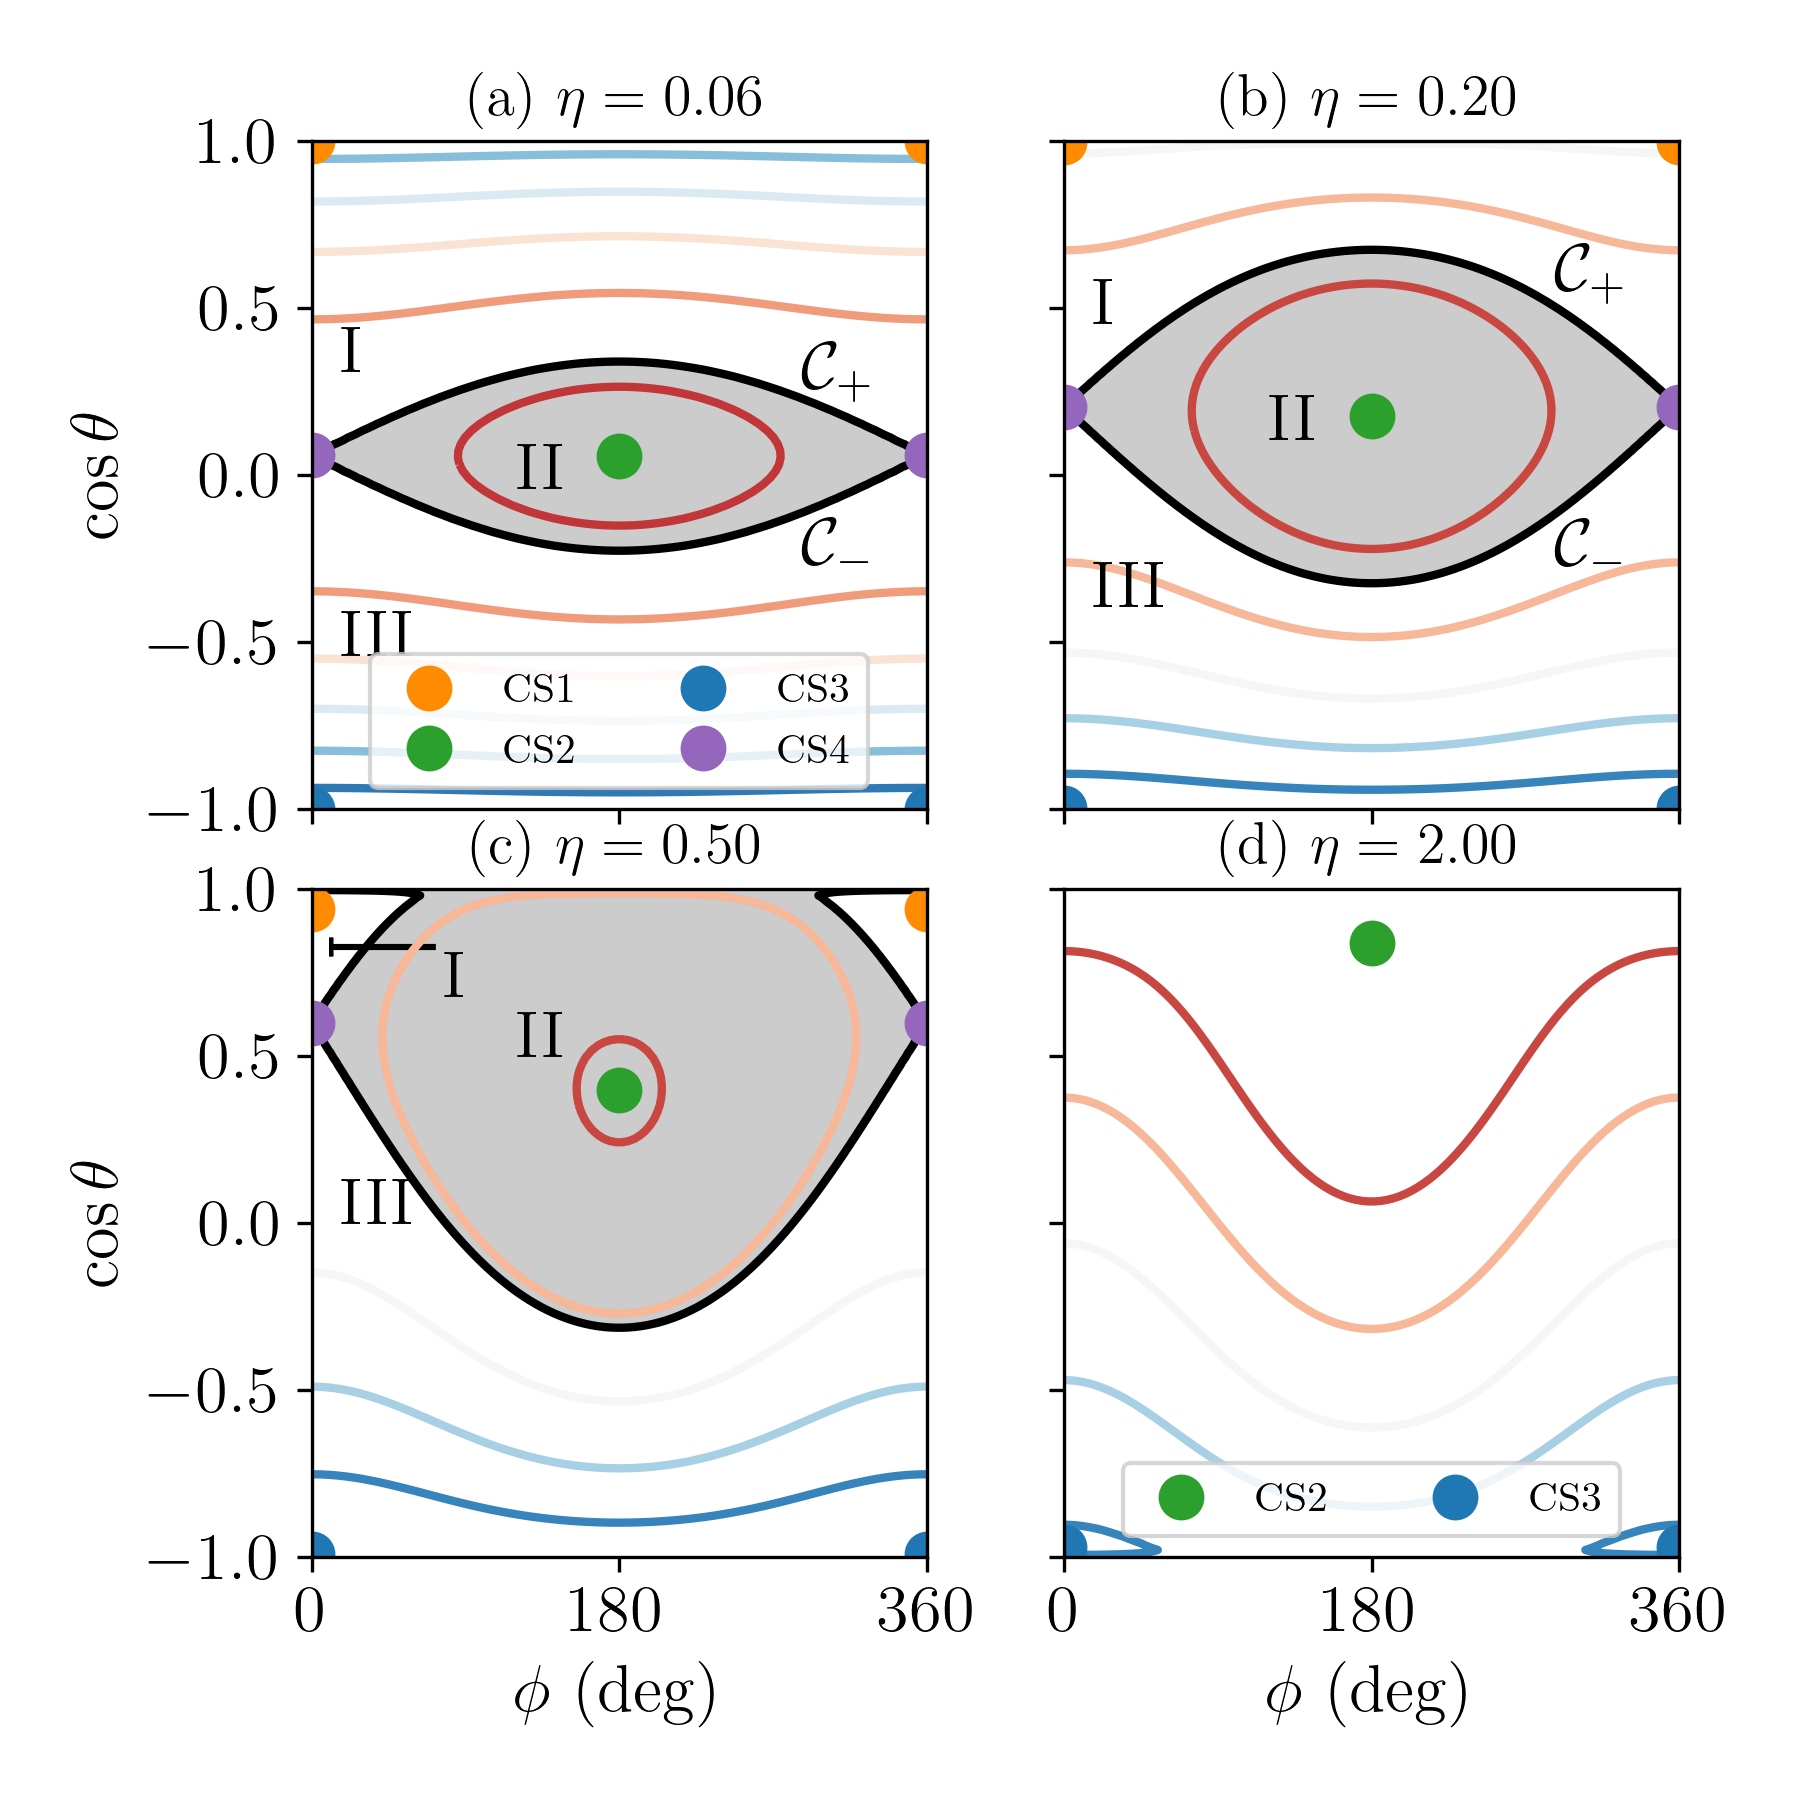
\includegraphics[width=0.6\columnwidth]{1contours20.png}
    \caption{Contour plots of the Cassini State Hamiltonian,
    Eq.~\eqref{eq:H}, for a few different values of $\eta$.}\label{fig:contours}
\end{figure}

\section{Tidal Dissipation and Resonance Capture}

\textbf{Key point:} Tidal dissipation causes the system to deviate from the
perfectly Hamiltonian evolution above. Most interestingly, if the obliquity is
initially $> 90^\circ$, then tidal dissipation, as it damps the obliquity
towards $0^\circ$, will cause the system to evolve through the separatrix in the
top-left panel of Fig.~\ref{fig:contours}. There is then some probability
associated with the outcome of this encounter; sometimes, it enters the
separatrix, and sometimes it does not. Qualitatively, this can be understood as
a small splitting of the separatrix induced by the tidal dissipation, which
permits some trajectories to enter the separatrix and rejects others.

Tidal dissipation occurs when the gravitational field of the host star raises a
small bulge in the fluid of the planet (like the Sun and moon raise bulges on
the Earth's oceans). The bulge both wants to point at the host star and wants to
rotate with the planet; these conditions are only in agreement when the planet
is \emph{tidally locked}, with zero obliquity and at spin-orbit synchronization.
Otherwise, dissipation ensues, where the obliquity will damp to zero and the
planet's spin rate will be driven to synchronization. We will focus on just the
first effect (obliquity damping) for simplicity and mostly discuss \S3 of
\citet{su2022dynamics}; see \S4 of \citet{su2022dynamics} for the treatment
including full tidal dissipation.

With a slow tidal obliquity damping torque, we can modify the equations in the
following prescriptive (read: made-up) way:
\begin{align}
    \rd{\theta}{\tau} &= \eta\sin I \sin \phi
        - \frac{1}{\tau_{\rm al}} \sin \theta, \label{eq:dqdt_toy}\\
    \rd{\phi}{\tau} &= - \cos\theta
        + \eta\p{\cos I + \sin I \cot \theta \cos \phi},\label{eq:dfdt_toy}
\end{align}
The idea is that tidal dissipation will damp $\theta$ on the characteristic
rescaled time $\tau_{\rm al} \gg 1$ (i.e.\ much slower than all precession
frequencies in the system).

For completeness, I must mention: the first way that tidal dissipation affects the
Cassini State dynamics is by changing the stability of the Cassini States; see
\citet{fabrycky2007cassini} for the most famous discussion of this. In simplest
terms, any tidal dissipation turns CS3 from a stable fixed point into a source,
while sufficiently strong tidal dissipation does the same to CS2; CS4 remains a
saddle point (unstable), and CS1 goes to zero obliquity (the tidally locked
state). But that will not be our focus today.

\textbf{We ask the simple question: for an arbitrary initial condition $(\theta,
\phi)$, what is the ultimate fate of the system?} This is a very easy question
to answer when $\eta > \eta_{\rm c}$: since only CS2 and CS3 exist (bottom-right
panel of Fig.~\ref{fig:contours}), and CS3 is unstable to tidal dissipation,
everything ends up at CS2. When $\eta < \eta_{\rm c}$, two more cases can be
solved straightforwardly:
\begin{itemize}
    \item If the initial condition is in Zone I (labelled on
        Fig.~\ref{fig:contours}; roughly the set of prograde $\theta < 90^\circ$
        initial conditions), then tides will drive the system to CS1, the only
        stable equilibrium in this region of phase space.

    \item If the initial condition is in Zone II, tides drives the system to CS2
        instead.

    \item \textbf{But if the initial condition is in Zone III}, no tidally
        stable equilibria can be reached without encountering the separatrix. So
        we must study what happens during this encounter.
\end{itemize}
This is summarized in Fig.~\ref{fig:outcomes}.
\begin{figure}
    \centering
    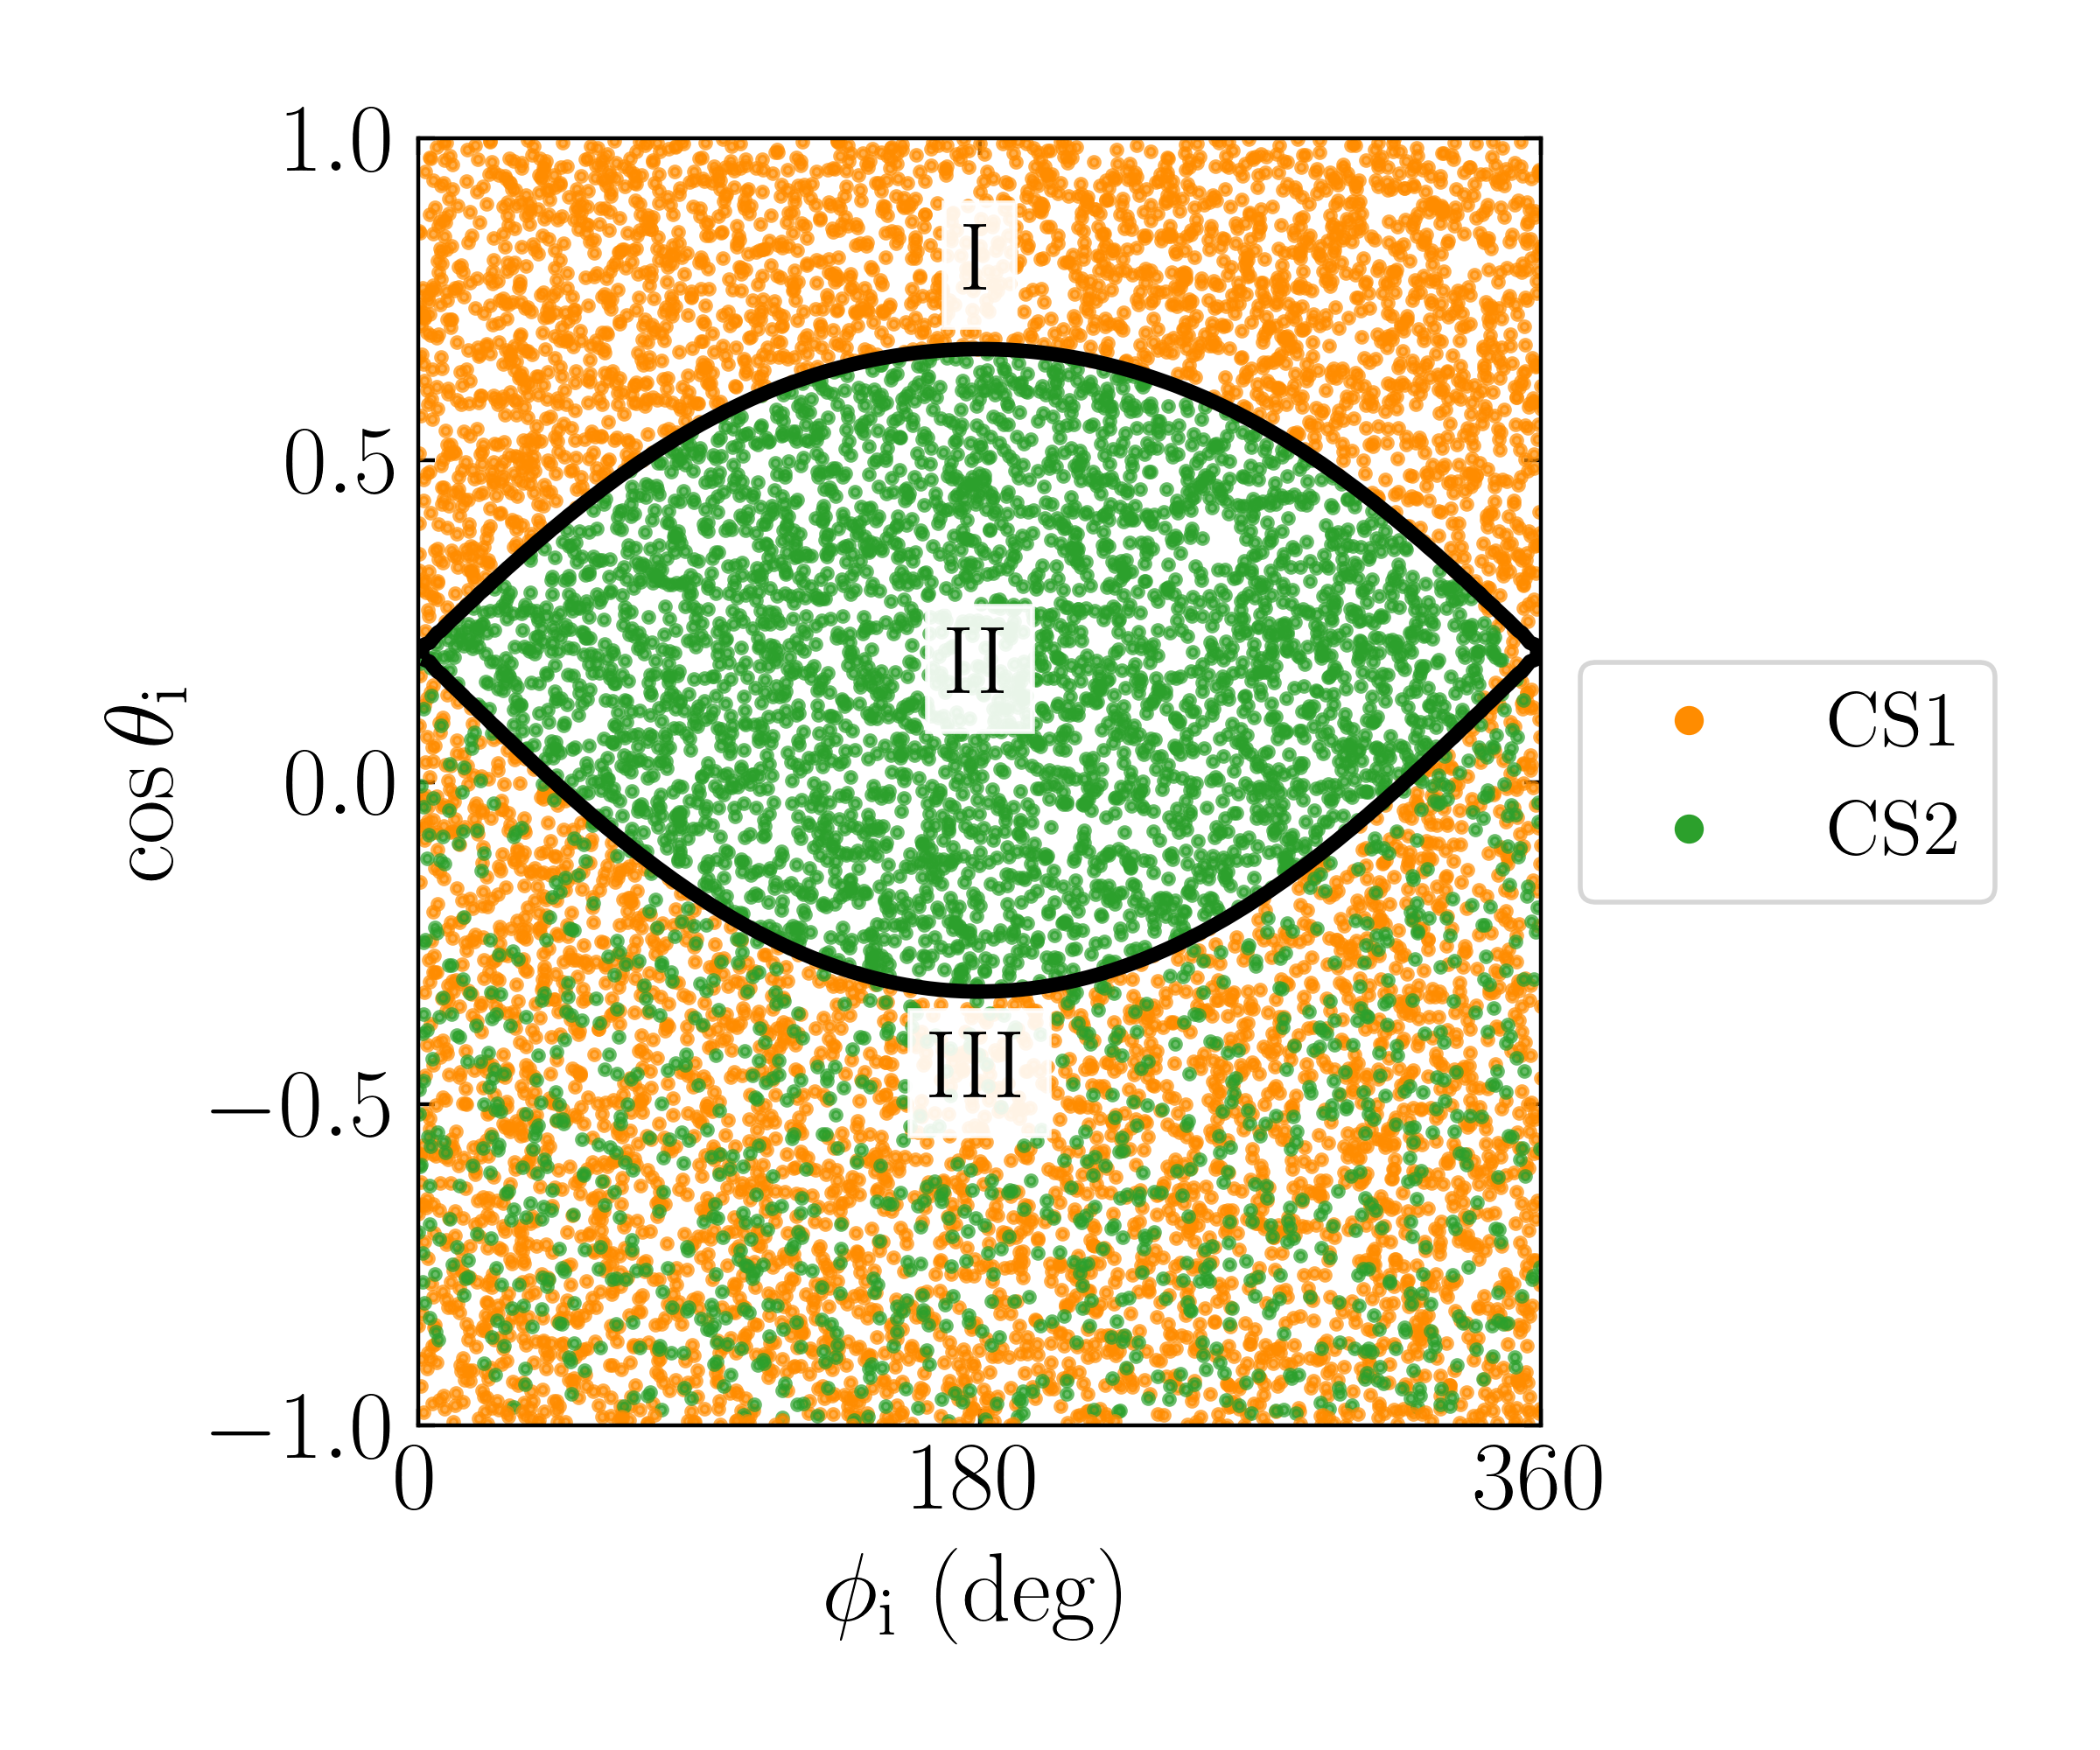
\includegraphics[width=0.5\columnwidth]{3stats3_5_0_2.png}
    \caption{Results of numerical experiments, where each dot is an initial
    condition that is integrated until it can be identified as reaching CS1
    (orange) or CS2 (green). Note the seemingly-probabilistic outcome of
    trajectories in Zone III.}\label{fig:outcomes}
\end{figure}

\subsection{Critical Orbits: Graphical Picture}

For reference, for this entire section, we keep Fig.~\ref{fig:manifolds} on our
minds.
\begin{figure}
    \centering
    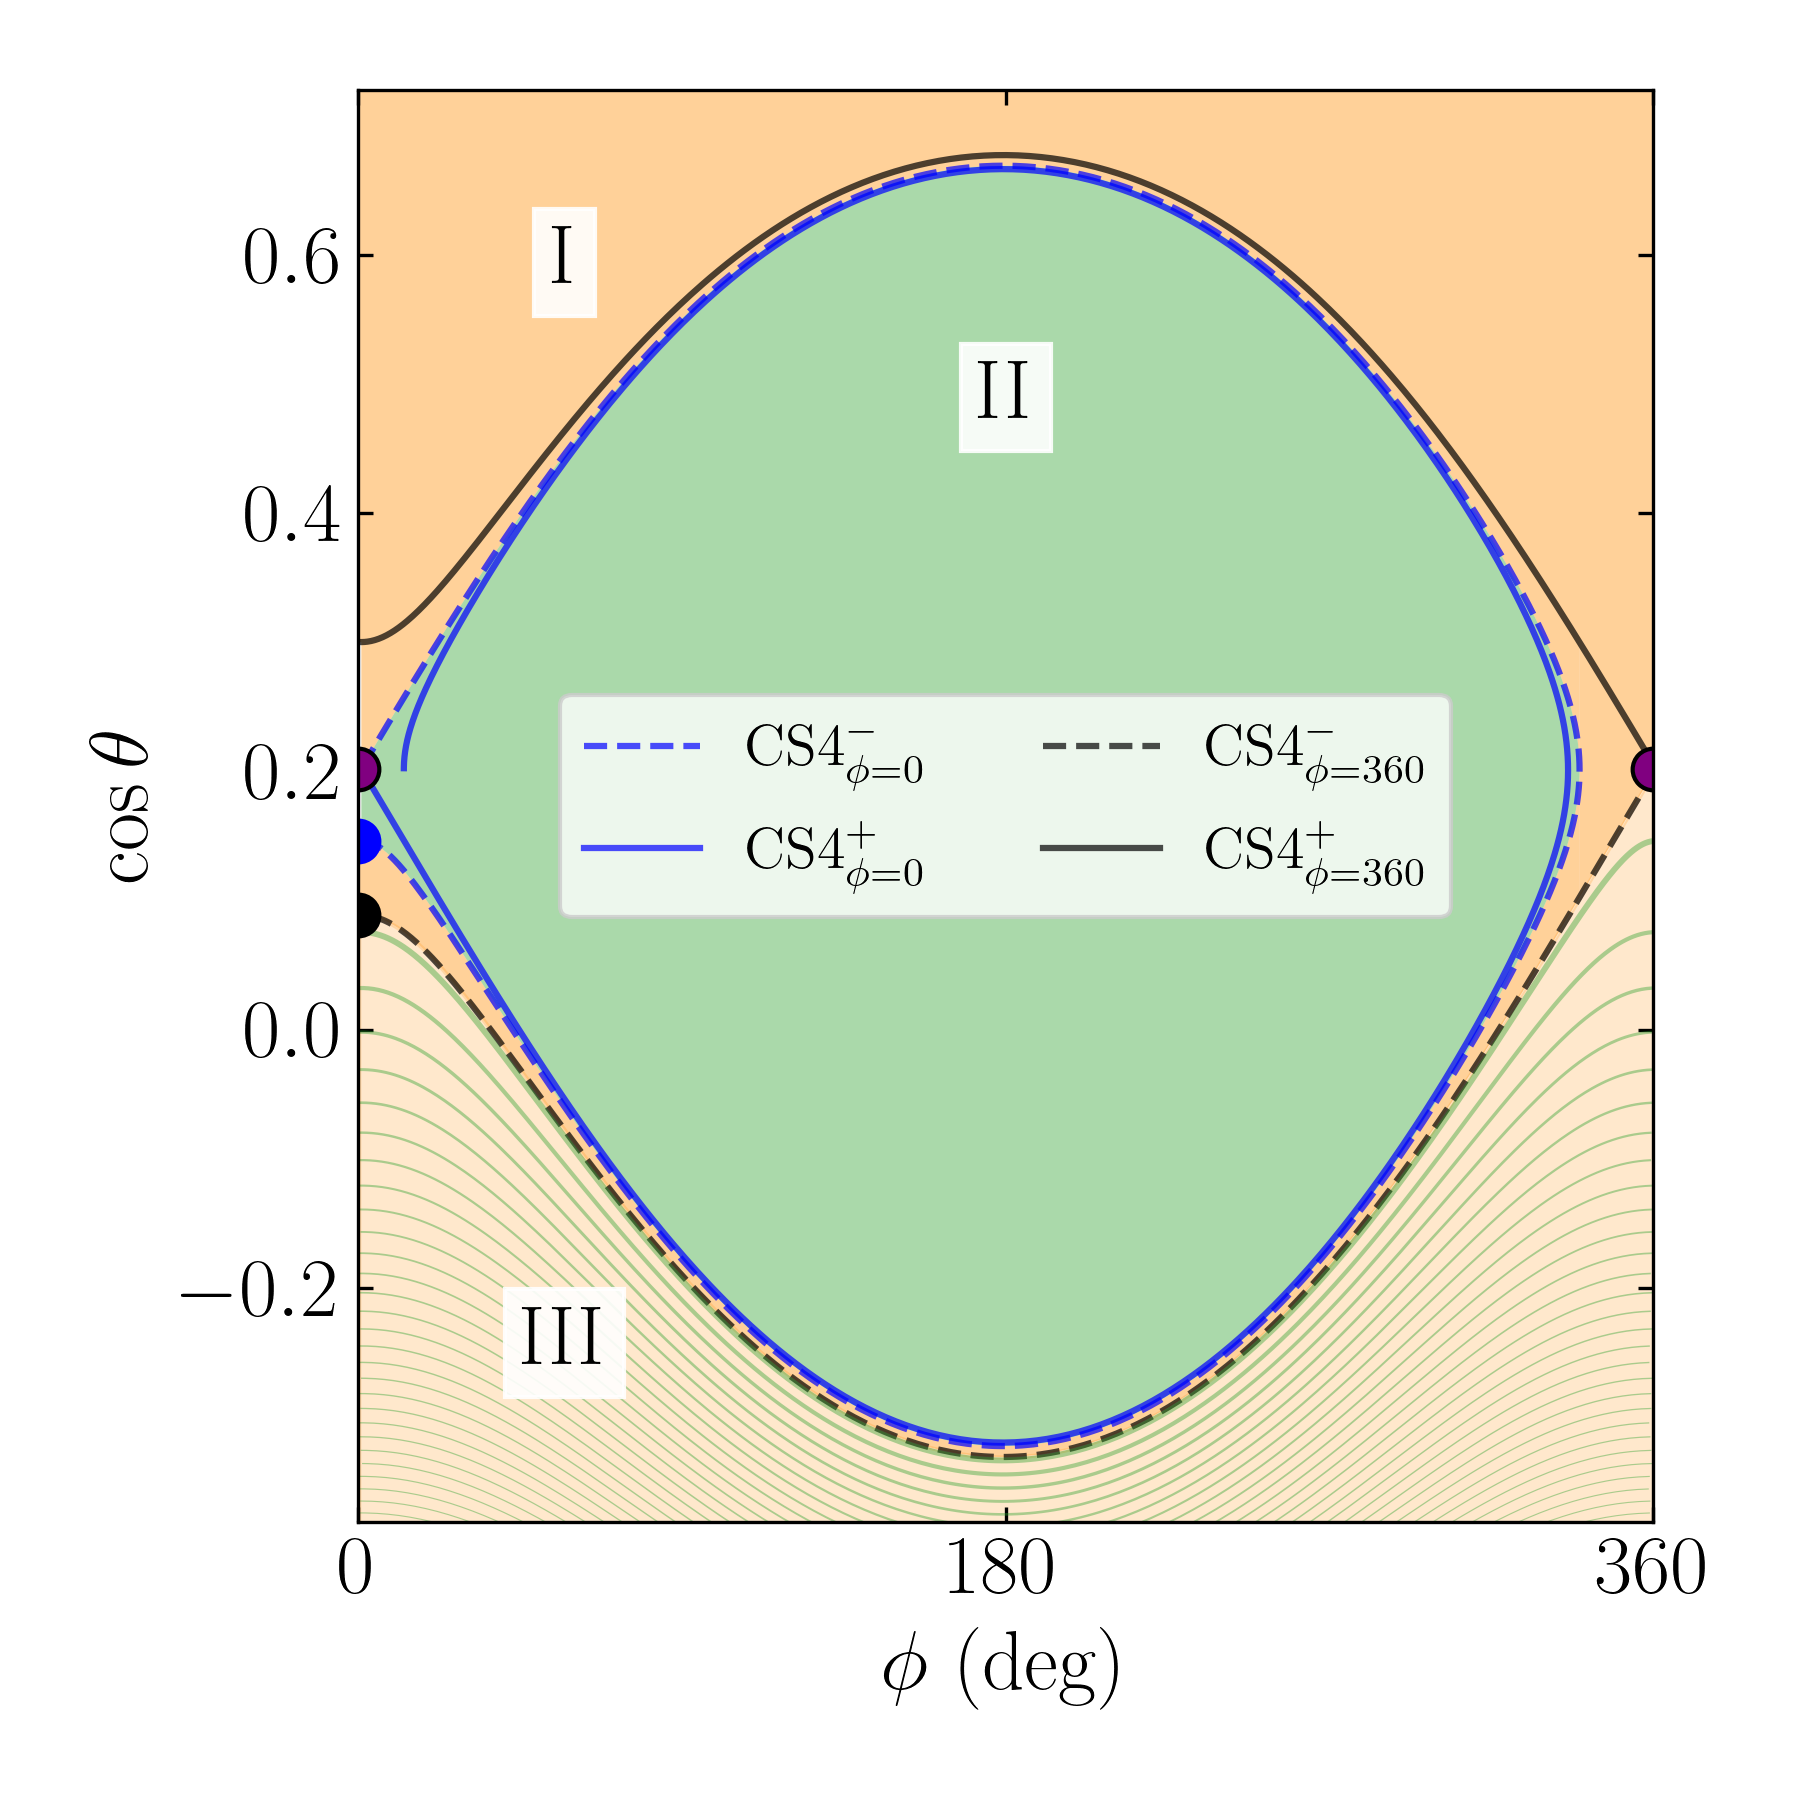
\includegraphics[width=0.8\columnwidth]{6manifolds0_20.png}
    \caption{Plot of the critical orbits / manifolds under the effect of tidal
    dissipation. Orange colored regions will tidally evolve towards CS1, and
    green regions to CS2. The notation CS4$_{\phi=0}^+$ denotes the orbit
    starting at CS4 (the saddle point) and $\phi = 0$ evolved forwards in
    time. Compare to Fig.~\ref{fig:outcomes}.}\label{fig:manifolds}
\end{figure}

Let's imagine the evolution of a significantly retrograde (Zone III) initial
condition, as it evolves. For simplicity of discussion, let's assume that the
initial condition is at $\phi = 0$ (though of course, for any initial
condition, we can just wait a fraction of a precession cycle to reach this):
\begin{itemize}
    \item Current location: $\p{\cos \theta_0, 0}$. After a single precession
        cycle ($\phi=0 \to \phi = 2\pi$), the system would return to its initial
        $\cos \theta$ in the absence of tidal dissipation. Including tidal
        dissipation, $\cos\theta$ increases by a small amount $\Delta$ to $\cos
        \theta_1$.

    \item Current location: $\p{\cos \theta_1, 0}$.
        After a second precession cycle ($\phi = 2\pi \to \phi = 4\pi$),
        $\cos\theta$ increases by another $\approx \Delta$ to $\cos \theta_2$,
        now that it is $\approx 2\Delta$ higher than its initial value.

    \item Current location: $\p{\cos \theta_2, 0}$.

    \item \dots

        When does this process terminate? When, over the course of a
        precession cycle, the trajectory encounters the separatrix. Thus, this
        evolution changes character when:

    \item Current location: $\p{\cos \theta_N, 0}$. In the
        course of the next precession cycle, the trajectory encounters the
        separatrix.
\end{itemize}
What must the value of $\cos \theta_N$ be? There are two easy bounds to
establish:
\begin{itemize}
    \item Consider the critical value such that after one precession orbit, it
        exactly reaches the saddle point; this is denoted by the black circle in
        Fig.~\ref{fig:manifolds}. If we are below this value, we will experience
        one more precession cycle before separatrix encounter; $\cos \theta_N$
        must be above the black circle.

    \item However, $\cos \theta_N$ cannot be above the saddle point, because
        then on its previous precession cycle, it must have encountered the
        separatrix. Thus, $\cos \theta_N$ must be below the purple circle in
        Fig.~\ref{fig:manifolds}.
\end{itemize}

\textbf{We have thus established that, on the separatrix-crossing orbit, the
trajectory must start between the black and purple dots in
Fig.~\ref{fig:manifolds}.} Determining the outcome of this separatrix crossing
orbit requires identifying a second critical orbit. Consider the point obtained
by evolving the saddle point backwards in time along the \emph{top} of the
separatrix (blue dashed line in Fig.~\ref{fig:manifolds}), which terminates in
the blue dot. At this point, we can just ``color in between the lines'': points
that are connected to the interior of the separatrix can be shaded green, points
that are exterior can be shaded orange, and \textbf{the outcome of the
separatrix-crossing orbit depends on whether $\cos \theta_N$ is above/below the
blue dot.}

\subsection{Capture Probability: Perturbative Analysis}

Above, we have provided the essence of the dissipative capture probability
argument. Next, it only remains to calculate the distances between the curves.
We can do this with some simple perturbation theory on $H$, the value of the
unperturbed Hamiltonian (which would be conserved in the absence of tidal
dissipation). Denoting the top and bottom halves of the separatrix by
$\mathcal{C}_{\pm}$ (see Fig.~\ref{fig:contours}), we can find that
\begin{align}
    H_{\rm purple} &= H_{\rm CS4} = H\p{\cos \theta_{\rm CS4}, 0},\\
    H_{\rm black} &= H_{\rm CS4}
        - \int\limits_{\mathcal{C}_-}\rd{H}{t}\;\mathrm{d}t,\\
    H_{\rm blue} &= H_{\rm CS4}
        - \int\limits_{\mathcal{C}_-}\rd{H}{t}\;\mathrm{d}t
        - \int\limits_{\mathcal{C}_+}\rd{H}{t}\;\mathrm{d}t.
\end{align}
Since tidal dissipation is small, all three of these values are very near
$H_{\rm CS4}$. Thus, for any initial condition, its specific value of $H$ in the
interval $H \in \s{H_{\rm purple}, H_{\rm black}}$ is nearly uniformly
distributed. Thus, the probability of resonance capture into the separatrix is
given by the fraction of the interval that is captured:
\begin{align}
    P_{\rm cap} &= \frac{H_{\rm purple} - H_{\rm blue}}{
        H_{\rm purple} - H_{\rm black}},\\
        &= \frac{
            \int\limits_{\mathcal{C}_-}\rd{H}{t}\;\mathrm{d}t +
            \int\limits_{\mathcal{C}_+}\rd{H}{t}\;\mathrm{d}t
        }{\int\limits_{\mathcal{C}_-}\rd{H}{t}\;\mathrm{d}t}.
\end{align}
Next, we can identify that
\begin{align}
    \int\limits_{\mathcal{C}_{\pm}}
            \rd{H}{t}\;\mathrm{d}t
        &= \int\limits_{\mathcal{C}_{\pm}}
            \pd{H}{\cos\theta}\rd{\cos\theta}{t}
            + \pd{H}{\phi}\rd{\phi}{t}\;\mathrm{d}\phi,\\
        &= \int\limits_{\mathcal{C}_{\pm}}
            \p{\pd{\cos\theta}{t}}_{\rm tide}\rd{\phi}{t}\;\mathrm{d}t,\\
        &= \int\limits_{\mathcal{C}_{\pm}}
            \p{\pd{\cos\theta}{t}}_{\rm tide}\;\mathrm{d}\phi.
\end{align}

We next need to evaluate this integral, so we need the curves parameterizing the
separatrix, $\mathcal{C}_{\pm}$. Using Eq.~\eqref{eq:H} and evaluting at CS4, it
is easy to obtain that legs of the separatrix, described by the curve
$\cos\theta(\phi)$, is given by
\begin{equation}
    \p{\cos\theta}_{\mathcal{C}_{\pm}}
        \approx \eta \cos I \pm \sqrt{2\eta \sin I\p{1 - \cos\phi}}.
\end{equation}
Thus, we obtain that (note that $\mathrm{d}\phi$ has different signs along the
different legs of the separatrix)
\begin{align}
    \int\limits_{\mathcal{C}_{\pm}}
            \rd{H}{t}\;\mathrm{d}t
        &= \int\limits_{\mathcal{C}_{\pm}}
            \frac{1 - \cos\theta}{\tau_{\rm al}}\;\mathrm{d}\phi,\\
        &= \mp \frac{1}{\tau_{\rm al}}
            \int\limits_0^{2\pi}
                1 - 2\eta \sin I\p{1 - \cos \phi}
                    \mp 2\eta \cos I\sqrt{2\eta \sin I}\p{1 - \cos
                    \phi}\;\mathrm{d}\phi,\\
        &= \mp \frac{1}{\tau_{\rm al}}
            \s{2\pi\p{1 - 2\eta \sin I}
                \mp 2\eta \cos I\sqrt{2\eta \sin I}\p{4\sqrt{2}}},\\
    P_{\rm cap}
        &= \frac{16\eta\cos I\sqrt{\eta \sin I}}{
            2\pi\p{1 - 2\eta \sin I}}.\label{eq:pcap}
\end{align}
This works very well, as seen in Fig.~7 of \citet{su2022dynamics} (reproduced
here as Fig.~\ref{fig:pcap}).
\begin{figure}
    \centering
    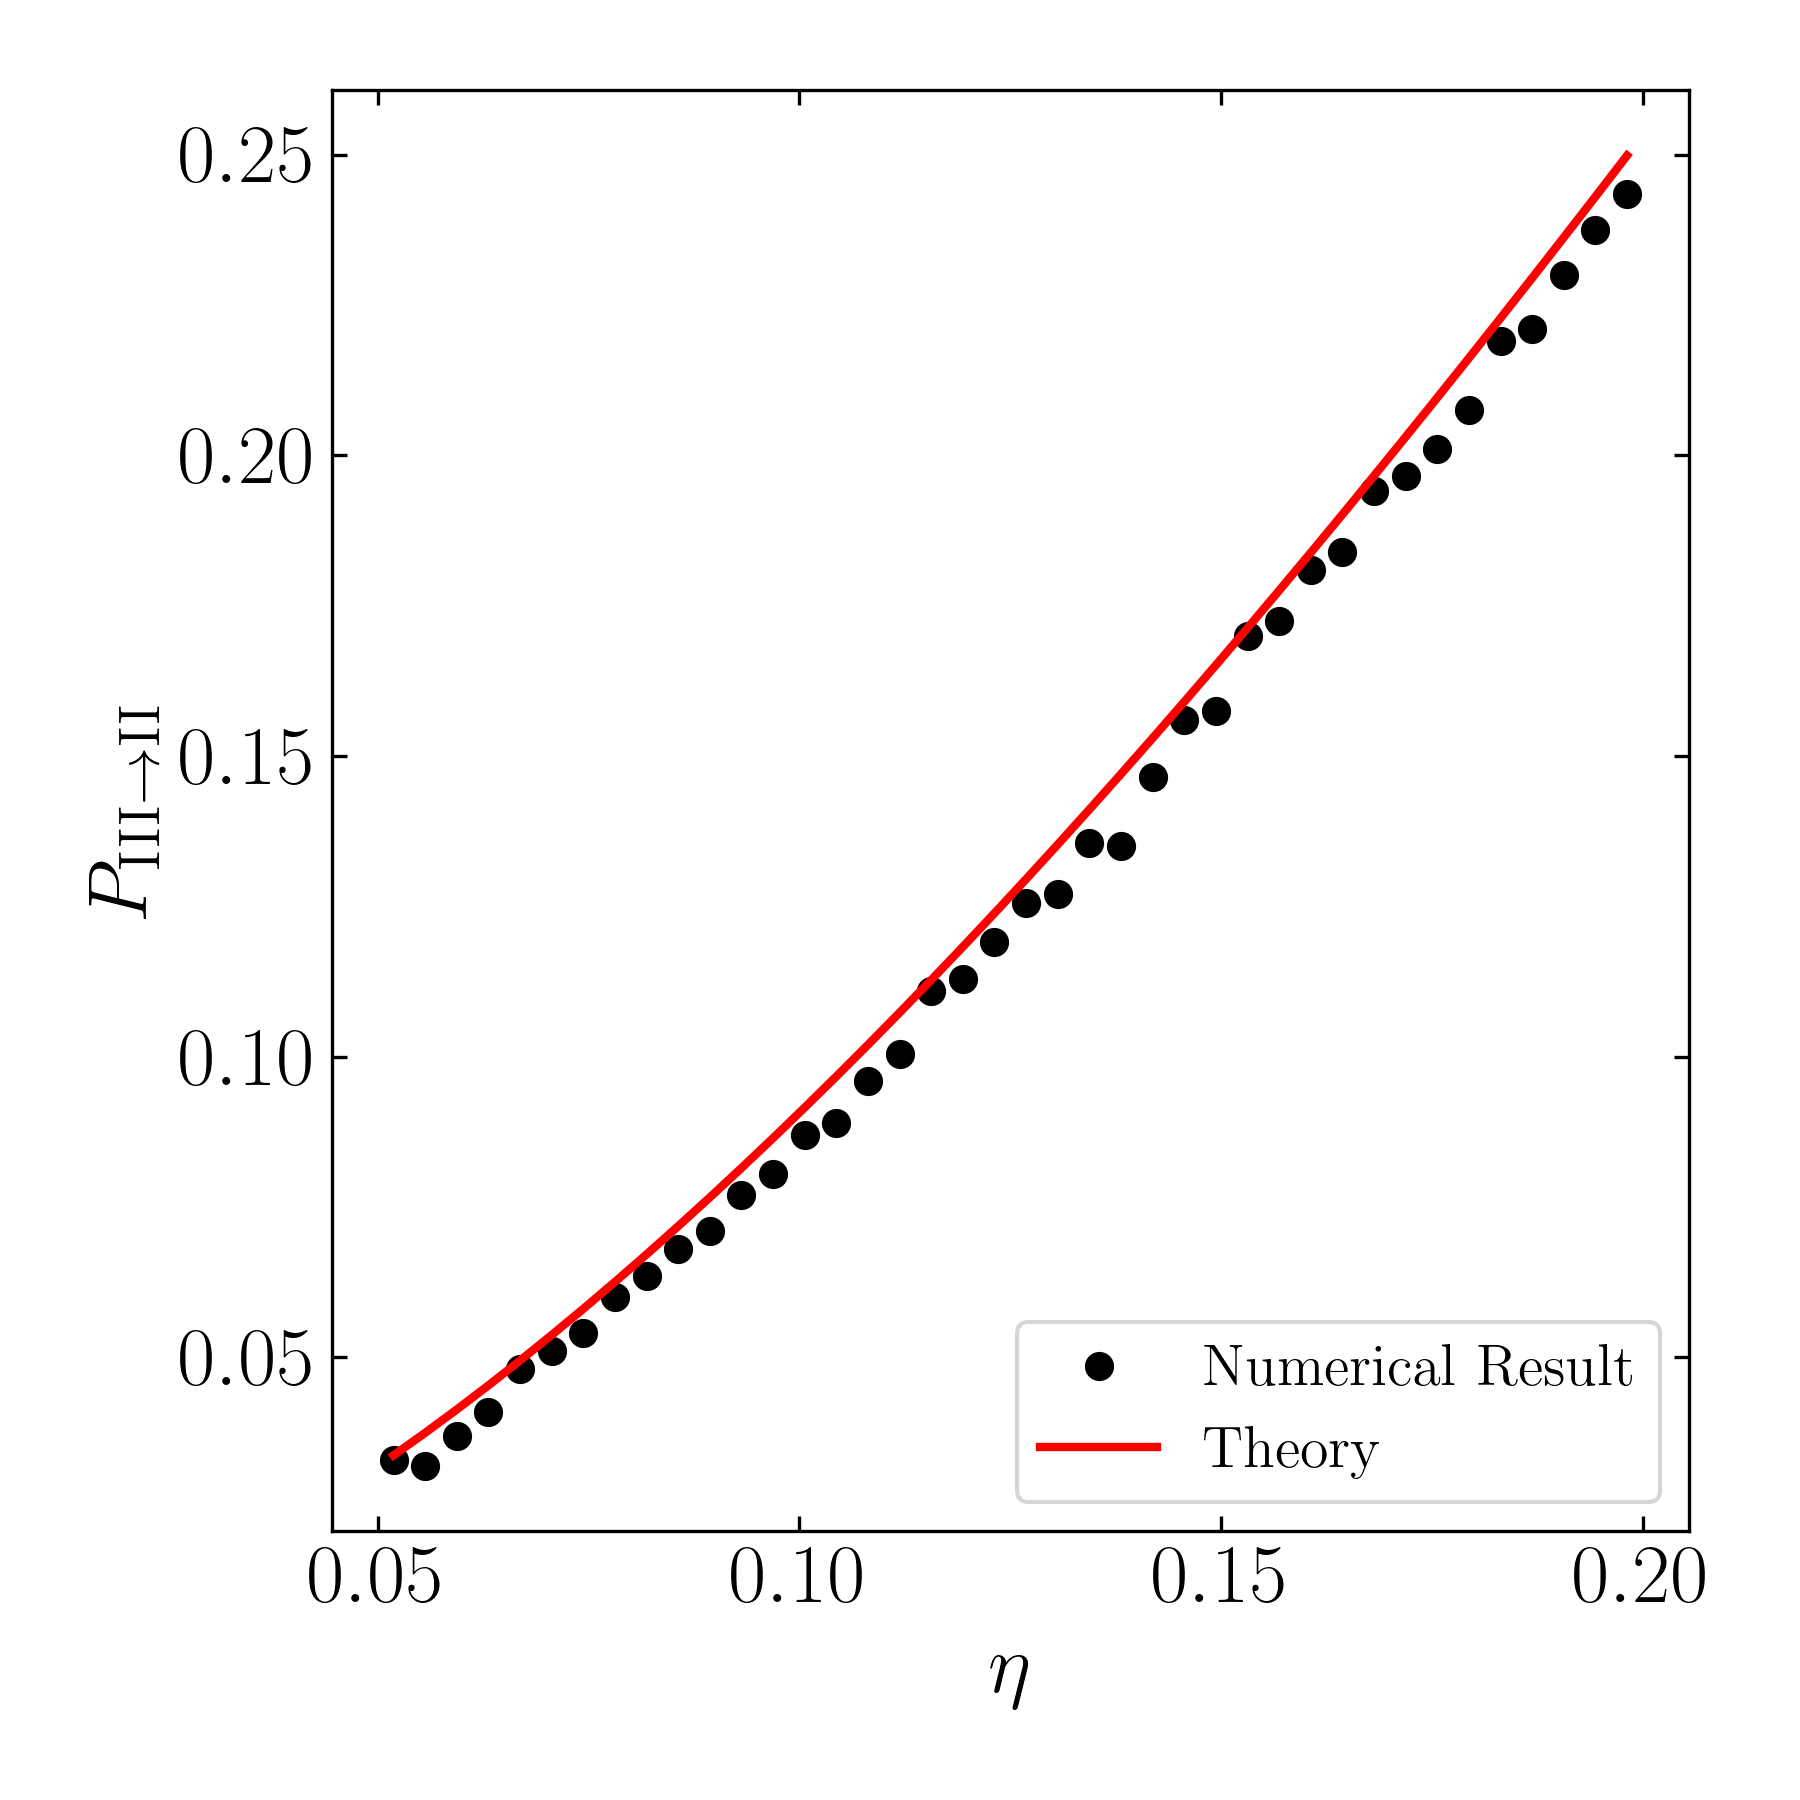
\includegraphics[width=0.5\columnwidth]{1hist_toy.png}
    \caption{Comparison of the capture probability Eq.~\eqref{eq:pcap}
    compared with numerical experiments.}\label{fig:pcap}
\end{figure}

\emph{Brief aside}, the computation of the distance between these critical
orbits is also known in the applied math community as \emph{Melnikov's method}
(\S4.5 of \citealp{guckenheimer2013nonlinear}), where it is used to compute the
distance between the \emph{stable and unstable manifolds} of the saddle point
(what I've called critical orbits above). In astrophysical dynamics, Melnikov's
integral is used instead to detect chaos traditionally (\S4.3.4 of
\citealp{2002morbidelli}).

\subsection{Relation to Adiabatic Resonance Capture}

Previously, you learned that when a Hamiltonian system has a parameter that is
adiabatically varied (e.g.\ pendulum with changing length), the probabilities of
transitions between two zones $i, j$ of phase space with areas $A_i, A_j$ is
given by
\begin{equation}
    P_{i\to j} = -\frac{\dot{A}_j}{\dot{A}_i}.
\end{equation}
This is simple to understand: since the Hamiltonian is varying adiabatically,
and phase space volume is an adiabatic invariant (Liouville's Theorem), the
probability of this transition occuring just comes down to where the phase space
volume lost by zone $i$ is going: how much of it is going to zone $j$, how much
to some other zone $k$.

Interestingly, this adiabatically varying Hamiltonian formalism and the
dissipative formalism I present above can be shown to be equivalent:
\citet{henrard1993adiabatic} gives a way of reducing a dissipative system to a
Hamiltonian one (with time dependence)! For the curious ones.

\bibliographystyle{apalike}
\bibliography{goodman_lecture}

\end{document}

